\documentclass[../main.tex]{subfiles}

\begin{document}

Earlier it was stated that the EMPIAR 10391 dataset exhibits conformational heterogeneity. This means that not all particles come from the same structure. In such cases, the alignment is performed against multiple reference volumes, so that for each particle not only the projection parameters are determined but also the volume that it originated from. In this section, we have used the experimental data of the EMPIAR-10391 dataset to test the effectiveness of our alignment algorithm to separate heterogeneous particles.

We have tested out algorithm using a resolution limit of $15 \si{\angstrom}$ and Wiener \gls{ctf} correction. The results shown in Figure \ref{fig:5:3d_classification} proof that the algorithm is able classify particles belonging to the second class, but it messes with the first class (the one without the drug attached), practically assigning images by chance to it. Although these results may not be promising, when compared to a Cryosparc refinement run with the same input data and default parameters, the results are better with our algorithm. 

\begin{figure}[htbp]
    \centering
    \begin{subfigure}[b]{.8\textwidth}
         \centering
         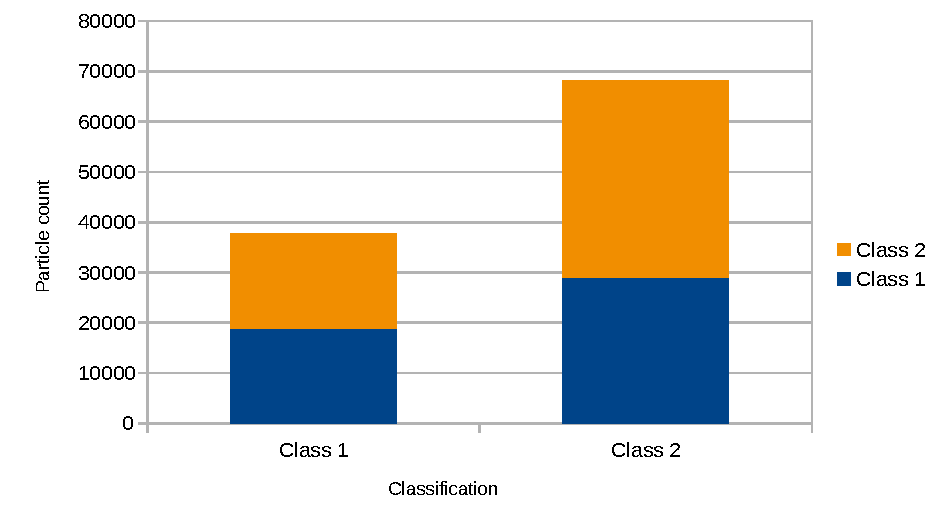
\includegraphics[width=\linewidth]{results/classification/cryosparc}
         \caption{Cryosparc}
    \end{subfigure}\\
    \vspace{2em}
    \begin{subfigure}[b]{.8\textwidth}
         \centering
         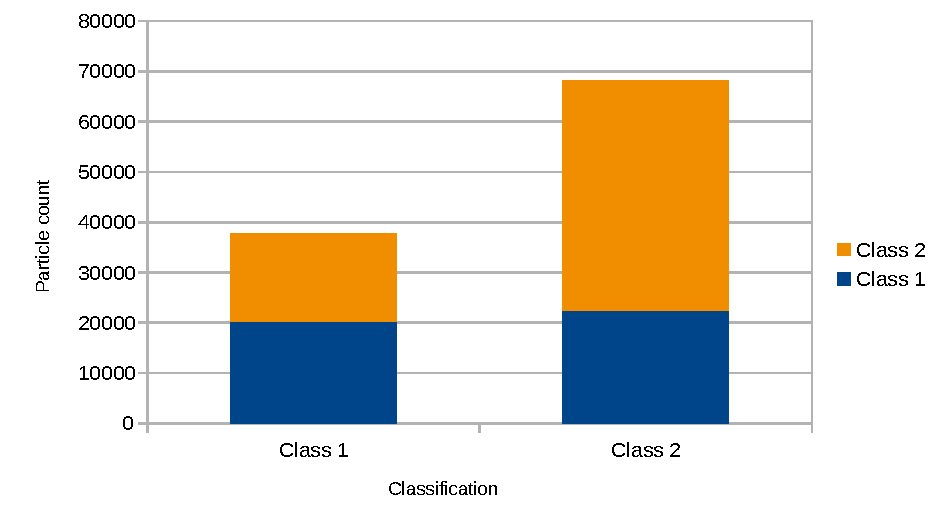
\includegraphics[width=\linewidth]{results/classification/swiftres}
         \caption{Swiftres}
    \end{subfigure}
    \caption{Comparison of 3D classifications of the EMPIAR-10391 dataset using Cryosparc and Swiftres}
    \label{fig:5:3d_classification}
\end{figure}

The former results can be potentially improved by performing the classification focusing on \gls{roi} defined around the area where the binding appears. This \gls{roi} is usually applied by masking the current volumes with a mask designed to leave that region.

\end{document}
